\chapter{Background}
\label{ch:background}
This chapter gives an overview over concepts and related works required for understanding the protocols and algorithms discussed in further chapters of the thesis.
\section{Preliminaries}

\subsection{Cryptography Concepts Overview}
The practice and study of mechanisms for secure communication is known as cryptography. Secure communication in digital communications is the assurance of message privacy between communicating parties, even when the communication channel is untrusted, and adversaries are present. Cryptography is the process of creating and evaluating protocols with the prime objective of assuring data confidentiality, integrity, and authenticity between communicating parties. The fundamental basis of cryptography are mathematical theory and computer science practice. Cryptographic algorithms are built around assumptions about computational difficulty. While it is theoretically conceivable to break such algorithms in a well-designed system, any adversary would find it infeasible in practice.
\par
Encryption is the operation of converting information (\textit{cleartext}) using cryptographic algorithms into a form (\textit{ciphertext}) that is unintelligible to the public or an adversary. The ciphertext can be restored to its original form by its intended recipient who owns the necessary cryptographic material to perform the decryption process. Encryption is a prominent and commonly utilized method to ensure confidentiality.
\par
On the other hand, integrity is the assurance that data has not been intercepted and modified by an adversary or corrupted in transit. Mainly, the approach to ensure data integrity is through mathematically compute a digital fingerprint for the data via hash functions. Subsequently, the digital fingerprint is attached to the data and sent to their designated party. The receiver verifies that the fingerprint corresponds to the data received, and thus the data integrity is proven.
\par
Cryptography is split into two main cryptosystems: Symmetric and Asymmetric cryptography.

\subsubsection{Symmetric Cryptography}
Symmetric cryptography, aka shared secret cryptography, relies in its operations on a private key that is shared between the communicating parties. In symmetric encryption, the shared secret is used for both encryption and decryption operations. Schemes for symmetric encryption are divided into two main categories according to how data is encrypted: Block ciphers and Stream ciphers.
Block ciphers scheme encrypts one fixed-size block of data at a time. In a block cipher, a given plaintext block will always encrypt to the same ciphertext when using the same key (i.e., it is deterministic) whereas the same plaintext will encrypt to different ciphertext in a stream cipher. Block ciphers can operate in one of several modes, e.g. CBC, CTR. AES is a well-known example of a secure block cipher algorithm.
\par
Stream ciphers scheme 
\subsubsection{Asymmetric Cryptography}

\subsection{Digital Certificates}
In the realm of public key cryptography, an \gls{ee} in possession of a key pair is able to encrypt, decrypt and sign data to and from other entities. This satisfies the confidentiality and integrity requirements of communication security. However, this is not sufficient to achieve the authentication and authorization goals
certificates, which are a requirement in several use cases. Authentication is the assurance that an entity is in fact who it claims to be, while authorization is the assurance that an entity has the privilege to communicate with a resource. Without authentication guarantees, a malicious third party can impersonate any other party in a communication channel or manipulate the messages between two communicating parties. Moreover, the intrusion cannot be detected. To address this problem, digital certificates were introduced.
\par
A digital certificate (aka public key certificate) is an electronic document that cryptographically binds a public key to the identity of an \gls{ee}. The certificate is cryptographically signed by a trusted third party that issues the certificate. In addition to including the public key and the digital signature, the certificate also contains information about the public key, the identity of its owner, and information about the certificate issuer. The party that wishes to authenticate itself presents its digital certificate to its counterpart. To validate a certificate, the receiving party has to trust the certificate issuer. If the issuer is trusted, then its public key is used to verify the certificate's signature and as a result trust the presented certificate.
\par
To be able to use digital certificates in a scalable environment like the internet, a trusted large scale infrastructure that allows for the generation, storage, and distribution and revocation of certificates is required.
Although not the only one, the X.509 standard \cite{x509} is the most commonly used for specifying digital certificates format and \gls{pki}. It is an product of International Telecommunication Union (ITU). X.509 certificates are widely used in many internet protocols, including TLS. Therefore, X.509 is considered a pillar of network security. Currently, there are three versions of X.509, the most recent of which is simply known as X.509 version 3. In addition to the certificate identifiers and attributes, optional extensions have been added to the newest version, which can be tagged as critical and thus must be handled by the recipient, or can be ignored otherwise. In the X.509 \gls{pki}, a \gls{ca} is an entity responsible for handling end entities request to generate a certificate for their public keys from the \gls{pki}. The requests are known as \gls{csr}. The \gls{ca} verifies the identity of the \gls{ee} and checks the attributes of the \gls{csr} subsequently decides whether to issue and sign a certificate to the requester or not. In the X.509 PKI, the \gls{ca} is a trusted third party and the issued certificate is dubbed an \textit{\gls{ee} certificate}. Nevertheless, the \gls{ca} needs to have a certificate to identify itself. In a \gls{pki} there are several \glspl{ca} where they are organized in a hierarchical architecture. At the top level, there are the \textit{Root \gls{ca}} which have self-signed certificates as they are the highest authority. Root \glspl{ca} issue certificates to \glspl{ca} in the same level (cross certification) or in lower levels. Lower level \glspl{ca} are named \textit{intermediate \glspl{ca}} which can issue certificates to end entities. Though end entities cannot use their certificates to issue other certificates. Another component of a PKI is the \gls{ra}. A \gls{ca} can delegate some of its functionality to a \gls{ra}. A \gls{ra} lies between the \gls{ca} and the \gls{ee}, in addition, it is usually in proximity to the \gls{ee}.
\par
\gls{pki} provide methods for certificate revocation. Naturally, a certificate is only valid for a limited time due to various constrains. There are numerous critical reasons why its validity must be terminated sooner than allotted due to various threats, and hence the certificate must be revoked. For example, compromise of \gls{ee} or a trusted \gls{ca} private key. Wohlmacher \cite{revocationSurvey} provides a survey study of revocation methods that gives a good overview of the main revocation methods.

\subsection{Bootstrapping}
The term ``Bootstrapping" is used in a spectrum of contexts including Computing, Law, Finance\footfullcite{bs-wiki}. It is inspired from the late idiom ``to pull oneself up by one's bootstraps" which means to succeed or elevate yourself without any outside help. In the context of Networking, bootstrapping is an initial procedure between pledges (unconfigured devices) which intend to communicate with a network for the first time. Its goal is to provide the device with the required information that enables it to establish subsequent secure communication channels with the desired network. Such information can be certificates, configurations, and metadata. More on bootstrapping in chapter \ref{ch:secureBootstrapping}.


\subsection{Bootstrapping Voucher Artifact}
While bootstrapping, the pledge must be able to authenticate the network attempting to take control of it, hence assigning ownership is critical for bootstrapping techniques. Defined in \cite{rfc8366}, a voucher is a signed document that identifies the cryptographic identity of the domain that a pledge should trust. The goal of the voucher is to allow for a authorize a zero-touch imprinting of the pledge on the registrar of a domain. The voucher is signed by a manufacturer's \gls{masa}. The voucher artifact is a JSON formatted document which is included and signed in a CMS structure \cite{rfc5652}. The artifact data model is formally described by a YANG \cite{rfc7950} module in \cite[Section~5.3]{rfc8366}. Essentially, the main purpose of a voucher is to securely convey a certificate to the pledge with which it can authenticate the owner's domain registrar. The said certificate is found in the ``pinned-domain-cert" attribute of the voucher. 
\par
Vouchers can be classified into two types: nonced and nonceless vouchers. Nonced vouchers contain the same nonce specified by the pledge in its submitted voucher request. Nonces provide mitigation against replay attacks as they are not reusable. On the other hand, Nonceless vouchers may be reusable. Their validity is dependent on their lifetime which may vary. A voucher's lifetime is specified by its ``expires-on" attribute. 
Since voucher are non-revocable artifacts, the specification recommends short-lived vouchers rather than long-lived vouchers with the possibility to renew a voucher by reissuing it. The specification points out that the renewal process should be a lightweight process, as it ostensibly only updates the voucher's validity period. There may also exist nonceless vouchers without expiration times, however, they are advised against as they provide their bearer with extreme control over the pledge. Lastly, some pledges may not have the capability of understanding time, such pledges must not use vouchers with time constrains.

\subsection{Certificate Enrollment}
Certificate enrollment is the process where an \gls{ee} requests and obtains a digital certificate from a \gls{pki}. The process starts by the \gls{ee} submitting a \gls{csr} to the \gls{ca} or \gls{ra} of the \gls{pki} which the \gls{ee} intends to obtain a digital certificate from. Several protocols \cite{rfc7030,rfc4210,rfc8894,rfc5272} were proposed to address certificate enrollment.
\par
For certificate enrollment protocols, it is mandatory for \gls{ee} to authenticate messages from \glossary{pki} entities. This is achieved by installing a root CA certificate on the \gls{ee} that enables it to authenticate the PKI entities. Nevertheless, provisioning such certificate to an EE is out-of-band of certificate enrollment protocols, but it is achievable through bootstrapping protocols. On the other hand, the \gls{pki} may authenticate \glspl{ee} using certificates they already posses or through private shared secrets.
\par
Some protocols, like \cite{rfc8894} require the EE to generate their own key pair locally, but some protocols, like \cite{rfc7030,rfc4210}, provide the possibility to generate the key pair for the EE during certification and transfer the keys to the EE during the process. In either case, the EE has to provide proof of possession of the private key, possibly through digital signature, decryption, or challenge-response.
Messages in certificate enrollment protocols have to be protected either by digital signatures or MACs.
\par
Certificate enrollment protocols generally realize a set of basic functionalities. These functionalities include certificate enrollment, certificate update and renewal, and certificate revocation. However, how each protocol implements a functionality can differ in its features. For instance, \cite{rfc5272} allows \glspl{ee} and/or \glspl{ra} to revoke \glspl{ee} certificates, while \cite{rfc8894} allows only \glspl{ca} to revoke certificates.
Different certificate enrollment protocols offer different functionalities. Some are only concerned with communication between \glspl{ee} and CA/RA, while others offer intra-PKI entities communications. For example, \cite{rfc4210} realizes cross-certification between \glspl{ca}.

\subsection{Protocol Formal Verification}\label{bg:pfm}
Formal verification is the application of mathematical procedures to confirm that a design complies with some clearly specified notion of functional correctness. In the lack of formal mechanisms for verification, security flaws may go unnoticed. On the other hand, formal verification approaches give a method for analyzing complex protocol in detail and prove the absence of large classes of attacks in a systematic fashion. Automated verification tools are programs built around a specific approach of formal methods with the goal of providing security guarantees for protocol execution employing the underlying cryptographic primitives, cryptographic protocols, and network systems. They help uncover protocol situations or vulnerabilities that contradict the intuitive assumptions underlying the construction of a protocol since they can analyze a large number of scenarios based on rigorous mathematical notions.
\par
Symbolic model checking is a protocol verification technique for determining if a protocol's finite-state model fits a set of requirements. Symbolic protocol analyzers effectively identify attacks, but they provide poorer security assurances than standard cryptographic proofs that account for probabilistic and computational concerns since they treat cryptographic constructions as perfect black boxes. \gls{ofmc} \cite{ofmc} is a symbolic analyzer for security protocols. The AVISPA Intermediate Format IF \cite{avispa} is OFMC's native input language. AnB \cite{AnB} is an intuitive Alice-and-Bob-style language that OFMC also supports. OFMC automatically converts AnB to IF. It performs protocol falsification and bounded session verification by exploring the transition system resulting from an IF specification. OFMC successfully employs two primary techniques: the lazy invader and constraint differentiation. The lazy invader is a symbolic representation of the Dolev-Yao intruder \cite{dolev1983security} that functions in a demand-driven manner. Constraint differentiation is a broad search-reduction approach that combines the lazy intruder with partial-order reduction principles.

\subsection{Key Derivation Function (KDF)} \label{backgroung:kdf}
A \gls{kdf} is a cryptographic algorithm that generates keying material that cryptographic algorithms can use. The function requires two sorts of input: a secret value, such as a key or a password, and other data. The core of a KDF is often built using a pseudorandom function, such as Keyed cryptographic hash functions. A key derivation function iterates an n-bit pseudorandom function and concatenates the outputs until L bits of keying material are generated. Each output receives a distinct value with each cycle, thus if one key is compromised, the risk is isolated to that key while preceding keys remain secure. \gls{nist} proposed recommended techniques to use pseudorandom-based \glspl{kdf} in \cite{chen2008recommendation}. 
\begin{figure}[hptb]
	\centering
	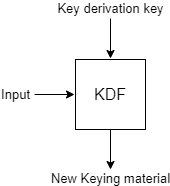
\includegraphics[scale=0.65]{Images/kdf.png}
	\caption{Key derivation function.}
	\label{fig:kdf}
\end{figure}

\section{Related Work}
\subsection{Key Continuity Management}
Peter Gutmann in \cite{gutmann-kcm-01} presented key continuity as a mechanism for assuring that the entity with whom a user is currently communicating is the same as the one they were previously communicating with.
Assuming the key resembles the identity of its user, the foundation for key management via key continuity is that once an entity has a remote entity's trustable key, it can validate later the remote entity's identity by confirming that they are still using the same key. The security mechanism relies on how long the key has been in service by its owner. The longer the key is witnessed to have been used, the more it is trusted by other entities. The research also proposed that an external authority manage the key continuity information. A key continuity external authority keeps track of how long a particular key has been used by a specific cryptographic service and responds to inquiries with that information. The document discusses key continuity in several security protocol use cases.
\par
However, the document does not precisely discuss authentication of keys at first use. Rather, the author has mentioned the possibility of users following the \gls{tofu} approach, or out-of-band means, for example, comparing key fingerprints over the phone. Moreover, He did not rule out utilizing digital certificates to verify public keys; nevertheless, he deemed it a more tedious, expensive, and manual process than \gls{tofu}. 

\subsection{Off-the-Record Protocol}
Consider the following scenario: Alice and Bob are alone in a room. Unless they are recorded, no one can hear what they are talking to one other. Therefore, no one knows what they are talking about until Alice and Bob tell them, and no one, not even Alice and Bob, can verify that what they are saying is true. \gls{otr} \cite{otr} aims to achieve the same form of secrecy in the field of instant messaging. The OTR protocol was first released in October 2004 by cryptographers Ian Goldberg and Nikita Borisov. At the time of writing, \gls{otr} is at version 3 \cite{otr3}. \gls{otr} provides a set of essential security features: Encryption, Authentication, Deniability, and forward secrecy.
\par
Abstractly, the protocol flow goes as follows. At first Alice and Bob establish a session encryption key through a \gls{dh} key exchange. Even though each party has established a shared secret, neither has a guarantee about authentication, i.e., no party is sure that the other party is whom it claims to be as a man-in-the-middle attack is possible. Each party owns a long-term public key for identity authentication. These keys are utilized discretely between the communicating parties to prove their identity to each other without sacrificing deniability to third parties. Alice and Bob generate signatures using their long-term private keys, enveloped in messages encrypted using the computed session key. Moreover, HMAC signatures are generated for messages to guarantee integrity as well as authenticity. Alice and Bob generate symmetric signing keys by passing the shared encryption key through hash functions. These signing keys are used to generate HMAC signatures. Next, parties can verify the signature received and consequently have the assurance of the party's identity at the other end of the channel. Assuming there was a man-in-the-middle, he would not be able to forge a signature for either party, and thus, signature verification would fail. Despite the use of digital signatures, they are used within an encrypted channel, and no other party can verify that both parties were communicating. After a message has been received and successfully decrypted, the sender publishes the message signing keys, and both parties delete their encryption keys and start over with the \gls{dh} key exchange to generate a new shared secret. Publishing signing keys enables outsiders to forge messages, enhancing the deniability feature for Alice and Bob. On the other hand, deletion of encryption keys ensures forward secrecy. Lastly, during the exchange of data messages, either Alice or Bob may employ the \gls{smp} \cite{smp} to detect impersonation or man-in-the-middle attacks.

\subsection{SoK: Secure Messaging}
Unger et al. \cite{unger2015sok} presented a comprehensive survey study where they used a methodology they've established to analyze and systematize current secure messaging solutions. Their survey valuably contributes towards an open standard for secure messaging by combining the most promising secure messaging features. The study looks at secure messaging solutions from academic research as well as real-world deployments, which identify innovative and promising ways that have already been implemented but are not covered in academic literature. The presented framework focuses on evaluating three main principles of the surveyed solutions: trust establishment, conversation security, and transport privacy.
For each, they evaluate the security, usability, and ease-of-adoption properties. However, security is the primary aspect relevant to our work.
\par
Trust establishment is defined as the procedure through which users ensure that they are communicating with the intended parties, i.e., a combination of long-term key exchange and long-term key authentication. While, transport privacy is concerned with preserving the privacy of users by obscuring metadata of messages during transit, such as the sender, receiver, and which conversation the message belongs to. Nevertheless, the aspect most relevant to our work is conversation security. It relates to protecting messages' security and privacy; and comprises the methods used to encrypt communications, the associated data, and the cryptographic algorithms employed. In addition to confidentiality, authentication, and integrity, discussed earlier, below are additional security properties. The following properties are relevant to two-party communication only as group communication is out of our scope.
\begin{itemize}
	\item \textit{Participant Consistency:} When one honest party accepts a message, all other honest parties are assured to have the same view of the participant list.
	
	\item \textit{Destination Validation:} When an honest party accepts a message, they may verify that they were included in the message's intended recipients list.

	\item \textit{Anonymity Preserving:} The underlying transport privacy architecture's anonymity characteristics are not jeopardized by the message exchange protocol.
	
	\item \textit{Speaker Consistency:} The order of messages transmitted by each participant is agreed upon by all participants. During the protocol, or after each message is transmitted, a protocol may execute consistency checks on blocks of messages.

	\item \textit{Causality Preserving:} It is possible to prevent showing a message before messages that are causally related to it in the implementation.
	
	\item \textit{Global Transcript:} All of the messages are displayed in the same order to all of the participants. It's worth noting that this presupposes speaker consistency.
	
	\item \textit{Deniability:} In some secure communications protocol use cases, deniability is a desired property. It refers to the inability of others to verify that a particular individual transmitted the data. However, if Bob receives a message from Alice, he can be confident that Alice sent it, but he cannot prove it to anybody else. Anyone can forge messages after a conversation to make them look like they came from them. However, if it is during a conversation, participants can rest assured that the messages they exchange are authentic and have not been modified by an intruder. Secure messaging protocols that offer deniability can assure the user that anyone can forge messages on their behalf after a conversation has ended, but not during a conversation. Deniability may be realized by conversation security protocols in a variety of forms. The authors define the following deniability-related features.
	
	\begin{itemize}
		\item \textit{Message Unlinkability:} If a judge believes a participant authored one message in a conversation, that does not mean they authored all of the messages.
		
		\item \textit{Message Repudiation:} Under the assumption that the judge does not have access to the accused participant's long-term secret keys, provided a conversation transcript, and all cryptographic keys, including session keys, there is no proof that any individual user authored a given message.
		
		\item \textit{Participation Repudiation:} There is no proof that the honest participant was in a conversation with any of the other participants, given the conversation transcript and all cryptographic key material for all but one accused participant.
		
	\end{itemize}
	\item \textit{Forward} and \textit{Future secrecy} are discussed later in chapter \ref{ch:postcomp}
\end{itemize}
Their study concluded a number of outcomes.
First, the usability and adoption of trust establishment solutions with solid security and privacy guarantees are low. However, other hybrid approaches that have not been thoroughly examined in the academic literature may give better trade-offs in reality.
Second, most of the stated conversation security properties are not mutually exclusive; nonetheless, combining protocol designs has considerable potential for improvement. For two-party conversation security, the most outstanding and promising solution of the bunch was the per-message ratcheting with resilience for out-of-order messages combined with deniable key exchange protocols, as implemented in Axolotl (now called the double ratchet algorithm), can be employed today at the cost of additional implementation complexity with no significant impact on user experience. 
Finally, transport privacy remains a challenging problem as it is difficult to solve without paying significant performance penalties. Among the analyzed solutions, no suggested approaches provided strong transport privacy properties against global adversaries while also remaining practical.

%	\item immediate decryption:
%		the fact that messages might arrive out of order or be lost entirely. Additionally, parties can be offline for extended periods of time and send and receive messages asynchronously. Given these inherent constraints, immediate decryption is a very attractive feature. Informally, it ensures that when a legitimate message is (eventually) delivered to the recipient, the recipient can not only immediately decrypt the message but is also able to place it in the correct spot in relation to the other messages already received. Furthermore, immediate decryption also ensures an even 	more critical liveness property, termed message-loss resilience (MLR) in this work: if a message is permanently lost by the network, parties should still be able to communicate
\subsection{The TESLA Broadcast Authentication Protocol}\label{bg:tesla}
Source authentication and integrity are among the most challenging aspects of protecting broadcast communication. In other words, receivers of broadcast data can verify that the received data originates from the claimed source and the data has not been modified en route. This difficulty is exacerbated by mutually untrustworthy receivers and unreliable communication settings in which the sender does not retransmit dropped packets. While many broadcast networks can effectively convey data to several recipients, they also make it easy for a malicious user to impersonate the sender and insert broadcast packets. This is known as a packet injection attack. Participants must use a broadcast authentication protocol to resist the attack, allowing receivers to verify that the alleged sender indeed transmitted the received packet. Nevertheless, using asymmetric cryptography to sign each message is a high overhead for time and bandwidth. Similarly, simply using \glspl{mac} does not solve the problem as any receiver with the shared secret can impersonate the sender and forge data.
\par
Perrig et al. \cite{perrig2003tesla} aimed to tackle the problem by proposing the \gls{tesla} protocol. \gls{tesla} inflicts low overhead for communication and computation while generating and verifying authentic information. Moreover, it is scalable to large numbers of receivers and tolerates packet loss. Nevertheless, \gls{tesla} requires the sender and the receivers to be at least loosely time-synchronized as well as the receiver or the sender is required to buffer some messages. Loosely time synchronization is that a receiver does not need to know the difference between the sender and the receiver’s time, however, it is only interested in an upper bound on the sender's time, or also know as the maximum time synchronization error. \gls{tesla} also relies on one-way chains which are repeated use of one-way hash functions. Similar in principle to KDF chains explained in section \ref{backgroung:kdf}. 
\par
In principle, the sender in \gls{tesla} generates a chain from an initial random secret key $s_\ell$ by iteratively applying the one-way hash function till the desired chain length is achieved. All intermediate keys generated are stored securely as well as the final key $s_0$. The final key is referred to as the commitment key. The sender divides the timeline into intervals while assigning each key to an interval. A key is used to generate \glspl{mac} for the messages sent during the specified time interval. However, keys are used in an opposite order to how they were generated, as depicted in figure \ref{fig:tesla}. During an interval, the sender uses the key to generate \glspl{mac} but key remains secret to the sender through out that interval. Meaning that receivers are unable to verify the \gls{mac} during that interval and also no malicious entity is able to forge a valid message. After the interval has passed, the sender publishes the now expired key for receiver to verify messages whose \gls{mac} was generated using that key. Receivers also verify the correctness of the disclosed key by inputting it into the one-way chain. If after a number of iterations the commitment key is reached $s_0$, then the key belongs to the expected chain and is valid.
\begin{figure}[hptb]
	\centering
	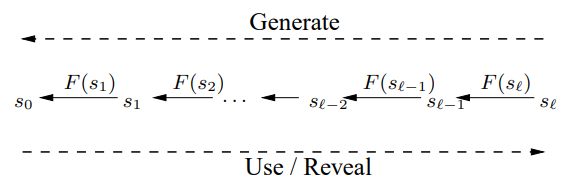
\includegraphics[scale=0.65]{Images/tesla.png}
	\caption{\gls{tesla} keys generation and usage \cite{perrig2003tesla}.}
	\label{fig:tesla}
\end{figure}
\par
Nevertheless, before authenticating messages with \gls{tesla} a receiver must be loosely time synchronized with
the sender, know the disclosure schedule of keys, and receive an authenticated key of the one-way key chain. The required information can be authentically obtained via digitally signed broadcast message, or over unicast with each receiver.
\par
Despite the security guarantees of the innovative approach, \gls{tesla} might not be suitable for some use cases due to the following limitations.
\begin{itemize}
	\item There is an initialization phase in which the first element of the hash chain must be transmitted to all recipients. In this step, authentication is accomplished using standard asymmetric cryptography. Furthermore, a new chain must be formed once the hash chain is depleted.
	\item The verification of a message or a set of messages is only possible once the next is received.
\end{itemize}

\subsection{A Survey of Key Bootstrapping Protocols}
Malik et al. \cite{bs-survey} provide a comprehensive survey study for a set of well-developed bootstrapping protocols in the context of \gls{iot}. They discuss the role of security and, in particular, key bootstrapping protocols at different layers of the \gls{iot} architecture. Next, they suggest a taxonomy for classifying key bootstrapping protocols, as shown in figure \ref{fig:bs-taxonomy}. The considered protocols are classified under the mentioned taxonomy and analyzed with the focus primarily on bootstrapping protocols based on asymmetric key distribution schemes. Lastly, they compare the surveyed key management schemes based on security and functionality features: Mutual Authentication, Forward Secrecy, resilience to key compromise impersonation, and resilience to replay attacks.
\begin{figure}[hptb]
	\centering
	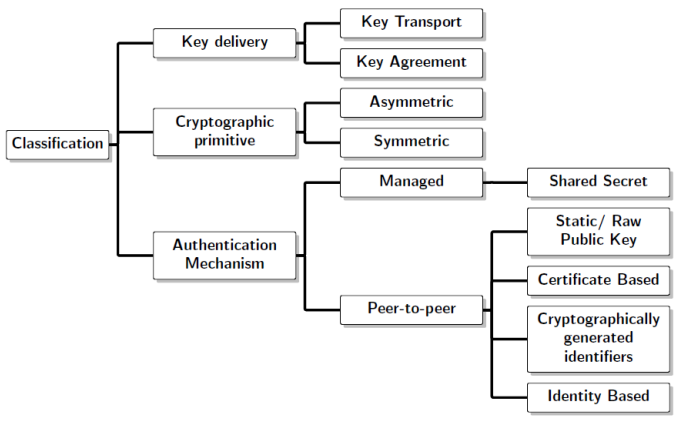
\includegraphics[scale=0.5]{Images/taxonomy.png}
	\caption{Taxonomy for classifying bootstrapping protocols \cite{bs-survey}.}
	\label{fig:bs-taxonomy}
\end{figure}

%\subsection{On post-compromise security}
%study post-compromise security in (classic) key exchange. Here, security shall be achieved even for sessions established after a full compromise of user secrets. This necessarily requires mixing user state information with key material that is newly established via asymmetric techniques, and is thus related to RKE.
